\subsection{Grafici di andamento}
Di seguito vengono riportati i grafici per ciascun documento con i valori rilevati. Si possono notare i valori limite di accettazione e ideale, che corrisponde anche al valore che il gruppo vorrebbe raggiungere nel prossimo periodo.

\begin{figure}[h]
	\centering
	
\includegraphics[scale=1]{Images/StudioDiFattibilità.JPG}
	\caption{Indice Gulpease \textit{Studio di Fattibilità}}
\end{figure}

\begin{figure}
	\centering
	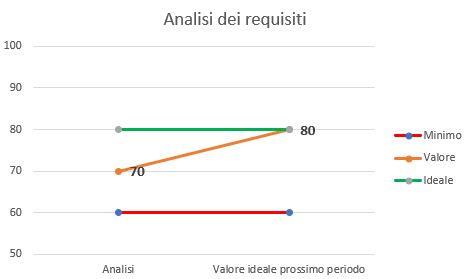
\includegraphics[scale=1]{Images/AnalisiDeiRequisiti.JPG}
	\caption{Indice Gulpease \textit{Analisi dei Requisiti}}
\end{figure}

\begin{figure}
	\centering
	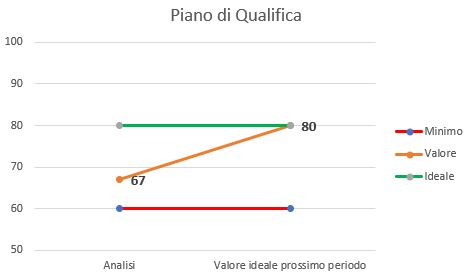
\includegraphics[scale=1]{Images/PianoDiQualifica.JPG}
	\caption{Indice Gulpease \textit{Piano di Qualifica}}
\end{figure}

\begin{figure}
	\centering
	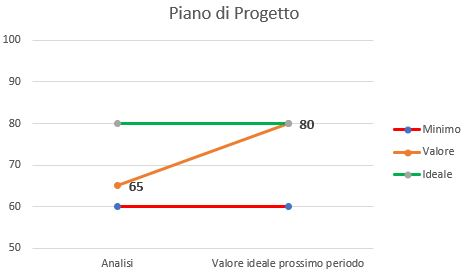
\includegraphics[scale=1]{Images/PianoDiProgetto.JPG}
	\caption{Indice Gulpease \textit{Piano di Progetto}}
\end{figure}

\begin{figure}
	\centering
	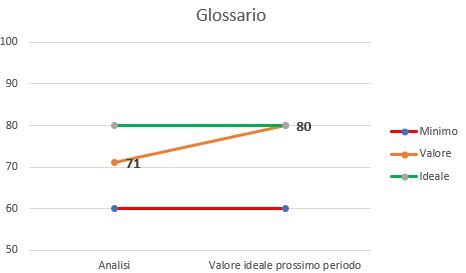
\includegraphics[scale=1]{Images/Glossario.JPG}
	\caption{Indice Gulpease \textit{Glossario}}
\end{figure}

\begin{figure}
	\centering
	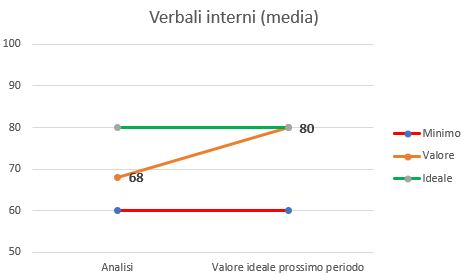
\includegraphics[scale=1]{Images/VerbaliInterni.JPG}
	\caption{Indice Gulpease medio dei verbali interni}
\end{figure}

\begin{figure}
	\centering
	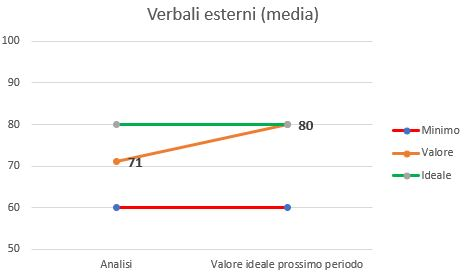
\includegraphics[scale=1]{Images/VerbaliEsterni.JPG}
	\caption{Indice Gulpease medio dei verbali esterni}
\end{figure}